\documentclass[xcolor=table]{beamer}

\usepackage[polish]{babel}
\usepackage[utf8]{inputenc}
\usepackage[T1]{fontenc}
\usepackage{listings}
\usepackage{lmodern}
\usepackage{textcomp}
\usepackage{subcaption}
\usepackage{etex}


\usetheme[language=polish]%
  {Goddard}

\newcommand{\filepath}{\texttt}
\newcommand{\command}{\texttt}
\newcommand{\email}[1]{\href{mailto:#1}{\texttt{#1}}}
\newcommand{\latexcode}{\texttt}
\newcommand{\parameter}[1]{\textlangle #1\textrangle}


\lstset{basicstyle=\ttfamily,keywordstyle=\color{goddardblue}\bfseries,commentstyle=\color{goddardblue!75}\itshape,columns=flexible}

\rowcolors{1}{goddardblue!50}{goddardblue!30}


\title{Szyfrowanie SMS’ów}
\subtitle{technologia oraz przegląd algorytmów}
\author{Bartłomiej Bułat\\
Tomasz Czarnik\\
Krzysztof Śmiłek\\}


\begin{document}

%==============================
\begin{frame}
  \titlepage
\end{frame}


%==============================
\begin{frame}
  \frametitle{Plan}
  \tableofcontents
\end{frame}


%=============================================================
\section{Wstęp}

\begin{frame}
  \frametitle{Wstęp}
 Krótkie wiadomości tekstowe potocznie zwane SMS (Short Message Service) na dobre zadomowiły się w większej części świata i stanowią dzisiaj jeden z popularniejszych kanałów komunikacji. \newline
\newline
W niniejszej prezentacji postaramy się przybliżyć technologię i słabości SMS oraz przeprowadzić przegląd wykorzystywanych metod szyfrowania wiadomości.  
% można tu umieścić komiks z XKCD lub dane z niego w porównaniu do całego Internetu 
% bathez: który komiks?
% miałem na myślie ten obrazek (dwie ramki z lewej), ale chyba jednak się nie nadaje: http://xkcd.com/802_large/
\end{frame}

\subsection{Zastosowania}
%==============================
\begin{frame}
  \frametitle{Zastosowania}

SMSy stosowane są między innymi do:
\begin{itemize}
\item wysyłania krótkich wiadomości i ,,czatów'',
\item aktywowania usług u operatorów komórkowych,
\item powiadomień od operatorów, banków i innych instytucji,
\item wysyłania bezpiecznych tokenów - haseł,
\item reklam i konkursów SMS,
\item sterowania urządzeniami. 
%kamerki szpiegowskie hehe
\end{itemize}
   
\end{frame}

%=============================================================
\section{Technologia}

%=============================================================
\subsection{Krótka historia GSM}
\begin{frame}[allowframebreaks]
  \frametitle{Krótka historia GSM}

  Pierwsza specyfikacja (GSM 900 Phase 1)
  \begin{itemize}
    \item \textbf{1982 r.} - powstanie instytutu Groupe Spécial Mobile, 2 lata
      później - projekt specyfikacji
    \item \textbf{1987 r.} - dyrektywa unijna o rezerwacji częstotliwości przez
      państwa członkowskie, rok później - specyfikacja GSM 900 Phase 1
    \item \textbf{1989 r.} - powstanie \emph{Europejskiego Instytutu Norm
      Telekomunikacyjnych (ETSI)}, przejecie prac nad standardem, rok później -
      domknięcie standardu i rozpoczęcie budowy infrastruktury
  \end{itemize}

  \framebreak

  Specyfikacja GSM Phase 2
  \begin{itemize}
    \item \textbf{1990 r.} - opracowanie specyfikacji GSM 1800 (DCS).
      Uwzględnienie przesyłania SMS-ów i danych.
    \item \textbf{1991 r.} - pierwsze połączenie telefoniczne w standardzie GSM
    \item \textbf{1993 r.} - uruchomienie DCS w Wielkiej Brytanii oraz pierwsze
      uruchomienie GSM poza Europą
    \item \textbf{1995 r.} - zakończenie prac nad standardem GSM Phase 2
  \end{itemize}
\end{frame}

%=============================================================
\subsection{Wiadomości SMS}

\begin{frame}
  \frametitle{Powstanie SMS}

  \begin{itemize}
    \item \textbf{1982 r.} - grupa GSM proponuje system wymiany wiadomości
      tekstowych miedzy stacjami nadawczymi lub za pomocą protokołu Message
      Handling System (wtedy bardzo popularnego)
    \item \textbf{1984 r.} - opracowanie koncepcji SMS-a jako wiadomości o
      długości 160 znaków wykorzystujący do przesyłania kanał informacyjny
      (nieużywany przez większość czasu komunikacji urządzeń) - przez Deutsche
      Telekom oraz France Télécom.
    \item \textbf{grudzień 1992 r.} - pierwszy SMS o treści ``Merry
      Christmas''
  \end{itemize}
\end{frame}

\begin{frame}
  \frametitle{Centra SMS}

  W pierwszych implementacjach SMS wiadomości były dostarczana kanałem
  informacyjnym bezpośrednio do odbiorcy. W późniejszych implementacjach stacji
  GSM dodano obsługę \emph{centr SMS (SMSC)}. Każdy wysłany SMS trafia do
  centrum które wysyła widomość do odbiorcy gdy ten znajduje się zasięgu sieci,
  jeśli nie wiadomość oczekuje do momentu zalogowania się odbiorcy. Jeśli minie
  czas ważności wiadomości SMS nie jest dostarczany.
\end{frame}

\begin{frame}
  \frametitle{Popularność SMS}

  \begin{center}
    \begin{figure}
      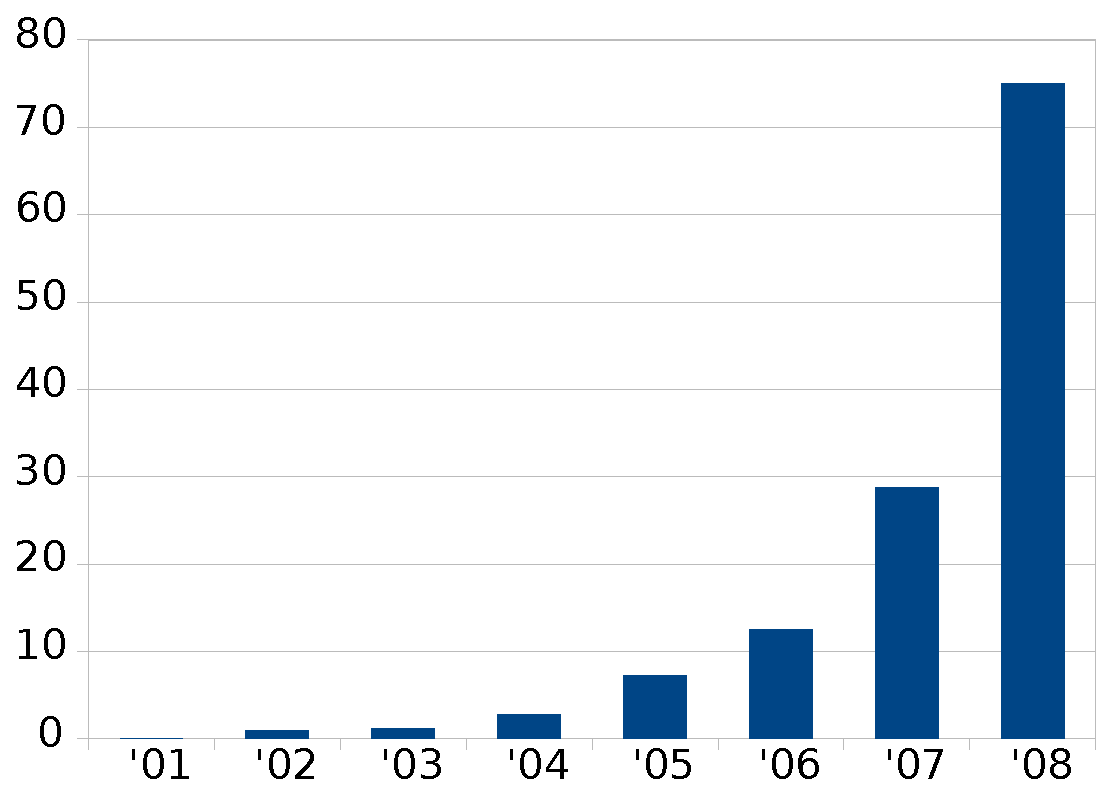
\includegraphics[width=0.7\textwidth]{sms_sent_monthly}
      \caption{Liczba wysłanych SMS-ów miesięcznie w USA w latach 2001 - 2008
      (w miliardach)}
    \end{figure}
  \end{center}
\end{frame}


%==============================
\subsection{Ograniczenia}
\begin{frame}[allowframebreaks]
  \frametitle{Liczba znaków}

  Początkowo SMS pozwalał na wysłanie 128 znaków (128 oktetów - 1024 bity).
  Następnie udało się rozszerzyć protokół do 140 oktetów (1120 bitów).
  Zmieniając kodowanie znaków na tzw. alfabet GSM, który używa 7 bitów na znak
  udaje się wysłać 160 znaków w jednej wiadomości.

  \textbf{Liczba 160 znaków} ma podłoże w badaniach przeprowadzonych na
  wiadomościach przesyłanych pocztówkami i przez dalekopisy. Analiza długości
  pozwoliła stwierdzić, że do tego typu komunikacji potrzeba ok. 150 znaków.
  Liczba natomiast 160 wynika ze specyfiki technologii.

  \framebreak

  \textbf{Alfabet GSM} - okrojona tablica ASCII do 127 pierwszych znaków, gdzie
  większość znaków sterujących została zastąpiona znakami z drugiej części
  tablicy ASCII.

\end{frame}
%=============================================================
\begin{frame}
  \frametitle{Problem znaków spoza alfabetu GSM}

  Współczesne urządzenia domyślnie wysyłają SMS w alfabecie GSM, jeśli jednak
  użyjemy znaku który znajduje się poza tym alfabetem (np. znaku z ogonkiem)
  wiadomość zostanie wysłana w kodowaniu LATIN-1 (dla polskiego alfabetu), które
  jest kodowaniem 8-bitowym, co zmniejsza pojemność SMS-a do 140 znaków.

  Jeśli chcemy użyć znaków z języków takich jak japoński, chiński, arabski czy
  cyrylicy należy użyć kodowania 16-bitowego UCS-2 co jednak redukuje pojemność
  SMS do 60 znaków.

  Niektóre nowoczesne telefony domyślnie przełączają się do kodowania UCS-2
  jeśli użyjemy znaku spoza alfabetu GSM.
\end{frame}

%==============================
\begin{frame}
  \frametitle{Łączone SMS (CSMS)}

  Istnieje możliwość wysłania wiadomości dłuższych niż 160 znaków. Jest to
  jednak tylko udogodnienie dla użytkownika, ponieważ SMS który przekroczy
  długość jest dzielony na części, a każda część zawiera nagłówek z informacją
  o serii wiadomości. Nagłówek w zależności od długości numeru referencyjnego
  zawiera 6 lub 7 bajtów. W nagłówku oprócz numeru referencyjnego serii
  wiadomości znajduje się również ilość oraz numer wiadomości w serii.

\end{frame}

%=============================================================
\subsection{Zagrożenia}
\begin{frame}
  \frametitle{Zagrożenia}

\begin{itemize}
  \item Podsłuch (sniffing) 
  \item Podszywanie się pod innego nadawcę (spoofing)
\end{itemize}

\end{frame}

\begin{frame}[allowframebreaks]
  \frametitle{Podsłuch}

  Podsłuch wiadomości SMS można podzielić na dwie kategorie: podsłuch
  komunikacji telefonu ze stacją bazową oraz podsłuch wiadomości przez wirusy w
  nowoczesnych telefonach komórkowych.

  Komunikacja GSM jest szyfrowana algorytmem A5/1, który nie jest pozbawiony
  wad. Opracowano już kilka rozwiązań do łamania kluczy szyfrujących tego
  algorytmu. Do podsłuchu tego rodzaju potrzebna jest też aparatura radiowa.

  \framebreak

  Wirusy na telefony komórkowe stały się popularne razem z systemem Android i
  iOS. Nawet stosując największe środki ostrożności może nie udać się ochronić
  przed niechcianym oprogramowaniem. Aplikacje podsłuchujące wiadomości
  przesyłają je korzystając z dostępnej sieci internet w telefonie. 
  Można się przed nimi zabezpieczyć instalując oprogramowanie
  antywirusowe lub stosując aplikacje do wysyłania szyfrowanych SMS-ów.
\end{frame}

\begin{frame}
  \frametitle{Spoofing}
  
  Istnieją dostępne w internecie usługi pozwalające wysłać wiadomości SMS jako
  dowolny nadawca. Można podać numer telefonu jak również tekst opisujący
  nadawcę. Głównym przeznaczeniem tej funkcjonalności jest komunikacja dostawcy
  usług z klientami, przesyłki reklamowe oraz SMS-y informacyjne (np. Wiadomość
  z ważnymi numerami telefonów po przekroczeniu granicy). Te możliwości SMS-ów
  mogą również zostać wykorzystane w celu wyłudzenia informacji lub pieniędzy
  od nieświadomego odbiorcy. Nie można automatycznie odfiltrować takich
  wiadomości dlatego jedynym sposobem na spoofing jest rozwaga i zdrowy
  rozsądek.

\end{frame}

%=============================================================
\section{Szyfrowanie}

%=============================================================
\subsection{Słownik T9}
\begin{frame}
  \frametitle{Słownik T9}
  Jest to podwórkowa ,,zabawa w szyfrowanie'' polegająca na tym, że całą wiadomość zapisujemy cyframi tak, jakbyśmy korzystali ze słownika T9 (poszczególnym cyfrom na klawiaturze telefonu są przypisane litery). Aby odszyfrować wiadomość odbiorca potrzebuje prześledzić literki na klawiaturze i domyśleć się wyrazów lub po prostu zanotować sobie ją na kartce obok i zacząć pisać nową wiadomość wpisując cyfry z pierwotnej wiadomości a słownik T9 będzie próbował odgadnąć wyrazy (można też skorzystać z drugiego telefonu). \newline
\newline
Dla przykładu wiadomość ,,Tajna wiadmość'' zakodowana zostaje do  postaci "825610942366672".

\end{frame}

%=============================================================

\subsection{Algorytm A5/1}

\begin{frame}
  \frametitle{Algorytm A5/1}
 Komunikacja GSM 
 wymagania, szyfrowanie symetryczne/asymetryczne i dlaczego (przede wszystkim kompresja i ograniczona liczba znaków )

\end{frame}

%=============================================================

\subsection{Protokół Diffiego-Hellmana}

\begin{frame}
  \frametitle{Protokół Diffiego-Hellmana}
	
Protokół uzgadniania kluczy Diffie-Hellman jest wykorzystywany w kryptografii
do ustalenia jednego klucza dla obu stron transakcji bez przesyłania żadnych 
poufnych informacji. Tak wygenerowany klucz jest później wykorzystywany przez
 algorytm symetryczny do szyfrowania połączenia między odbiorcą, a nadawcą. 
 Dzięki temu można zabezpieczyć transakcję przed podsłuchiwaniem przez osoby 
 postronne. Algorytm Diffie-Hellman nie jest odporny na atak 
 ,,man in the middle,, czyli ingerencję w komunikację między odbiorcą, 
 a nadawcą poprzez podmianę kluczy publicznych na własne.

\end{frame}

%=============================================================

\subsection{Algorytm OTR}

\begin{frame}
  \frametitle{Algorytm OTR}
	
Protokół OTR (Off The Record Protocol) został zaprojektowany przez kryptografów Iana Goldberga i Nikitę Borisova
specjalnie w celu kodowania wiadomości błyskawicznych (typu chat, SMS itp.).
Algorytm OTR używa kombinacji algorytmu klucza symetrycznego, 
protokołu Diffiego-Hellmana, funkcji skrótu SHA-1 i algorytmu AES. 

\end{frame}

\begin{frame}
  \frametitle{Algorytm OTR}

Zalety OTR:
\begin{itemize}
\item Szyfrowanie
\item Uwierzytelnianie - poprzez zastosowanie protokołu socialist millionaire 
osiągnięto ochronę na ataki typu ,,man in the middle,,
\item Zaprzeczalność - wiadomości w rozmowie nie posiadają podpisów cyfrowych,
zatem po zakończeniu rozmowy niemożliwym jest stwierdzenie, że konkretna 
wiadomość pochodzi od danej osoby
\item Poufność - wiadomości są szyfrowane jedynie tymczasowymi kluczami AES, negocjowanymi przy pomocy protokołu Diffiego-Hellmana. Ewentualne przechwycenie jakiegokolwiek długotrwałego klucza, nie skutkuje przechwyceniem żadnej z poprzednich rozmów.
\end{itemize}
\end{frame}

\begin{frame}
  \frametitle{Algorytm OTR}
  
Ograniczenia:
\begin{itemize}
\item brak obsługi czatu wieloosobowego
\item szyfrowanie tylko wiadomości (w planach jest też możliwość szyfrowania plików)
\end{itemize}
\end{frame}

%=============================================================
\section{Przegląd aplikacji szyfrujących SMSy}
%=============================================================

\begin{frame}
  \frametitle{uText Encrypted SMS}
	
	Platforma: Android\\
	uText Encrypted SMS pozwala na zaszyfrowanie wiadomości SMS 
wykorzystując istniejącego klienta wiadomości. Program używa protokołu 
	Diffiego-Hellmana w celu ustalenia tajnego klucza, który zostanie użyty 
	do zaszyfrowania wiadomości. Samo szyfrowanie wykorzystuje algortym AES (256bit).
	Do wymiany wiadomości wymagane jest:
	\begin{enumerate}
	\item zainstalowanie aplikacji u nadawcy i odbiorcy 
	\item zaakceptowanie klucza do wysyłania i odbierania wiadomości
	\end{enumerate}
	
\end{frame}
\begin{frame}
  \frametitle{uText Encrypted SMS}
    \begin{center}
        \begin{figure}
          \centering
            \begin{subfigure}[b]{0.4\textwidth}
               \centering
               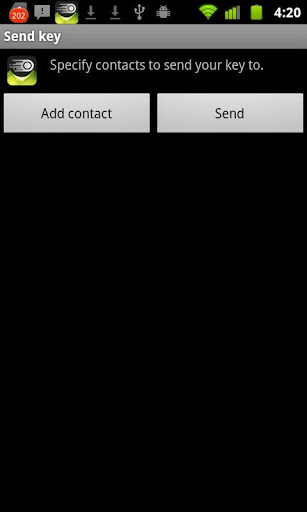
\includegraphics[width=\textwidth]{uText1}
              \caption{Wysyłanie klucza}
            \end{subfigure}
            \quad
             \begin{subfigure}[b]{0.4\textwidth}
              \centering
              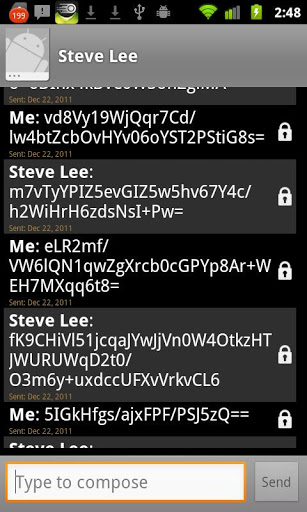
\includegraphics[width=\textwidth]{uText2}
              \caption{Zaszyfrowane SMSy}
            \end{subfigure}       
        \end{figure}
      \end{center}
\end{frame}

\begin{frame}
  \frametitle{TextSecure}
	
	Platforma: Android\\
	Aplikacja TextSecure to kolejna aplikacja pozwalająca na szyfrowanie 
	wychodzących wiadomości SMS. Jednakże proces szyfrowania odbywa się tutaj 
	za pomocą protokołu OTR. Aplikacja ma dodatkowo możliwość szyfrowania 
	wiadomości przechowywanych w pamięci telefonu poprzez użycie globalnego klucza.
		
\end{frame}
\begin{frame}
  \frametitle{TextSecure}
    \begin{center}
        \begin{figure}
          \centering
            \begin{subfigure}[b]{0.4\textwidth}
               \centering
               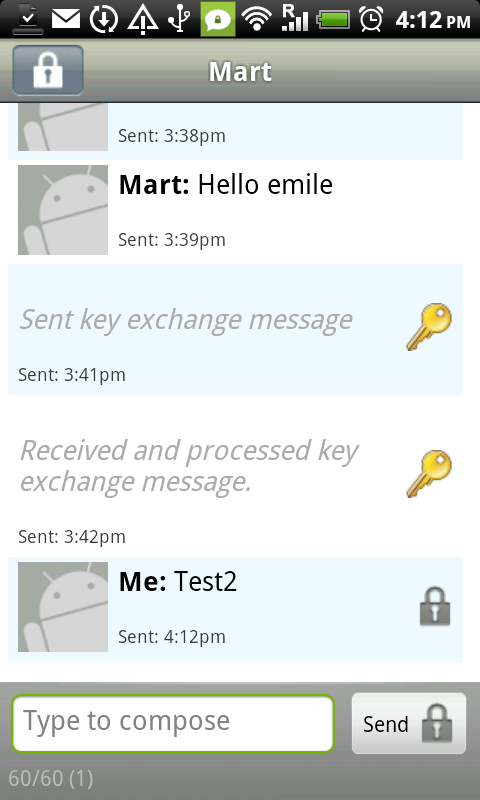
\includegraphics[width=\textwidth]{textsecure1}
              \caption{Wymiana kluczy}
            \end{subfigure}
            \quad
             \begin{subfigure}[b]{0.4\textwidth}
              \centering
              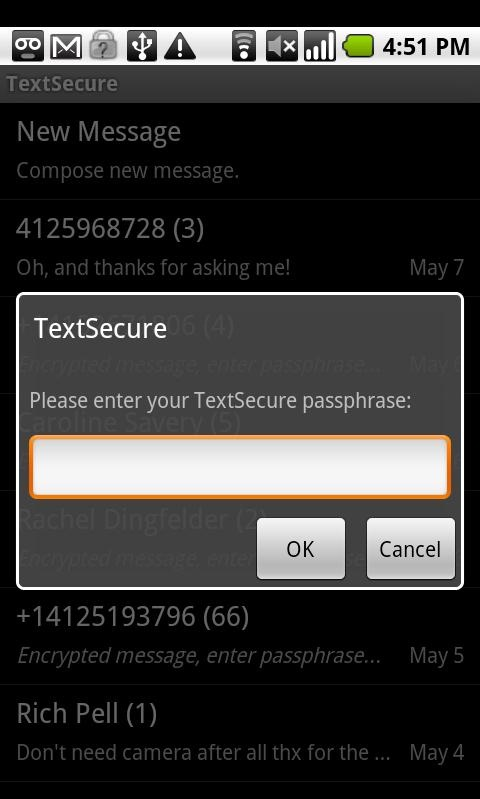
\includegraphics[width=\textwidth]{textsecure2}
              \caption{Podawanie klucza}
            \end{subfigure}       
        \end{figure}
      \end{center}
\end{frame}

\begin{frame}
  \frametitle{Secure Texting}
	
	Platforma: iOS\\
	Program ten jest bardzo prosty lecz wymaga znajomości hasła zarówno 
	od nadawcy jak i odbiorcy. SMS jest szyfrowany przez nadawcę przy użyciu 
	odpowiedniego hasła i przesyłany już w formie zaszyfrowanej. 
	Odbiorca jest zmuszony użyć tego samego hasła, aby odkodować wiadomość.
\end{frame}
\begin{frame}
  \frametitle{Secure Texting}
    \begin{center}
        \begin{figure}
          \centering
            \begin{subfigure}[b]{0.4\textwidth}
               \centering
               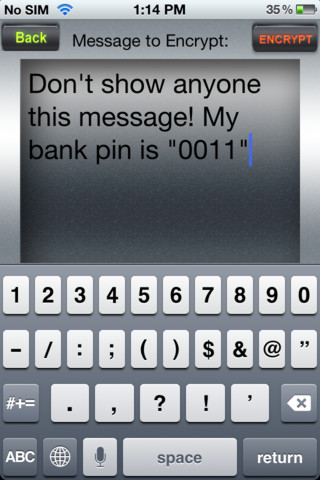
\includegraphics[width=\textwidth]{secure_texting_1}
              \caption{Wpisywanie SMSa}
            \end{subfigure}
            \quad
             \begin{subfigure}[b]{0.4\textwidth}
              \centering
              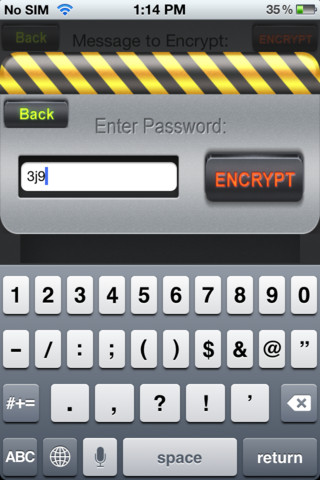
\includegraphics[width=\textwidth]{secure_texting_2}
              \caption{Podawanie klucza}
            \end{subfigure}       
        \end{figure}
      \end{center}
\end{frame}

%=============================================================
\section{Podsumowanie}

\begin{frame}
  \frametitle{Podsumowanie}
Spośród omawianych przez nas metod każda ma zalety, ale też pewne słabości.\\[\baselineskip] Przedstawione technologie i sposoby pozwalają łatwo wprowadzić szyfry i zaimplementować je np. w programie komputerowym korzystającym z modemu 3G lub działającym bezpośrednio na urządzeniu (np. pod systemem Android).

\end{frame}

\end{document}
